\documentclass[a4paper, 10pt]{article}
\usepackage{graphicx}
\begin{document}
\title{Mufasa Client Class}
\author{Merlijn Wajer}
\maketitle

\section{Introduction}

This is the official Mufasa Documentation.
The main purpose of this document is to provide a clear view on Mufasa's architecture.

\section{What is Mufasa?}

Mufasa is a project that aims to create two things, a GUI to create scripts, and a Mufasa Macro Library.
The Mufasa Macro Library (MML) will provide one with a way to control the mouse and keyboard, open files, open web pages, and capturing and analyzing images.
The GUI will use MML for most of it's features. Each script thread will also use a Client class.

\subsection{Simple feature overview}

Mufasa is:
\begin{itemize}
	\item Object Oriented. This means the code is generally more
		  readable, and easier to maintain.
	\item Free Software.\footnote{License here}
	\item MOAR
\end{itemize}

\section{Important Classes in MML}

\subsection{The Client Class}

The Client Class is the main Class, and is created to be able
 to run seperately from the User Interface, thus being thread safe.
The Client class is mainly designed to be a container for other classes.

\begin{figure}[h]
	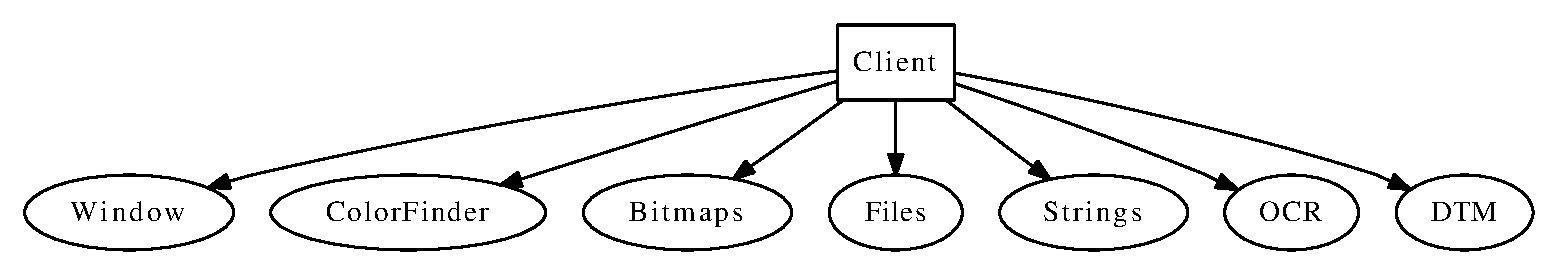
\includegraphics[scale=0.4]{Pics/Client_Classes}
	\caption{Classes that the Client contains.}
\end{figure}

\pagebreak

\subsection{The Window Class}

\begin{figure}[h]
	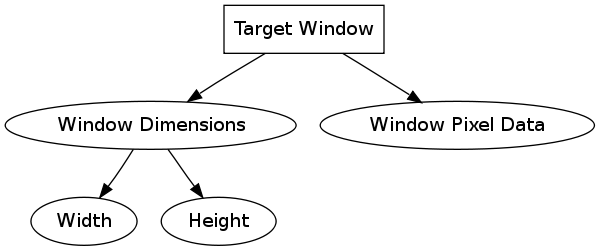
\includegraphics[scale=0.4]{Pics/Window}
	\caption{The structure of the Window class}
\end{figure}

The window class manages the core functionality for retreiving Window data, such as the actual pixels, position, or dimensions.

\begin{figure}[h]
	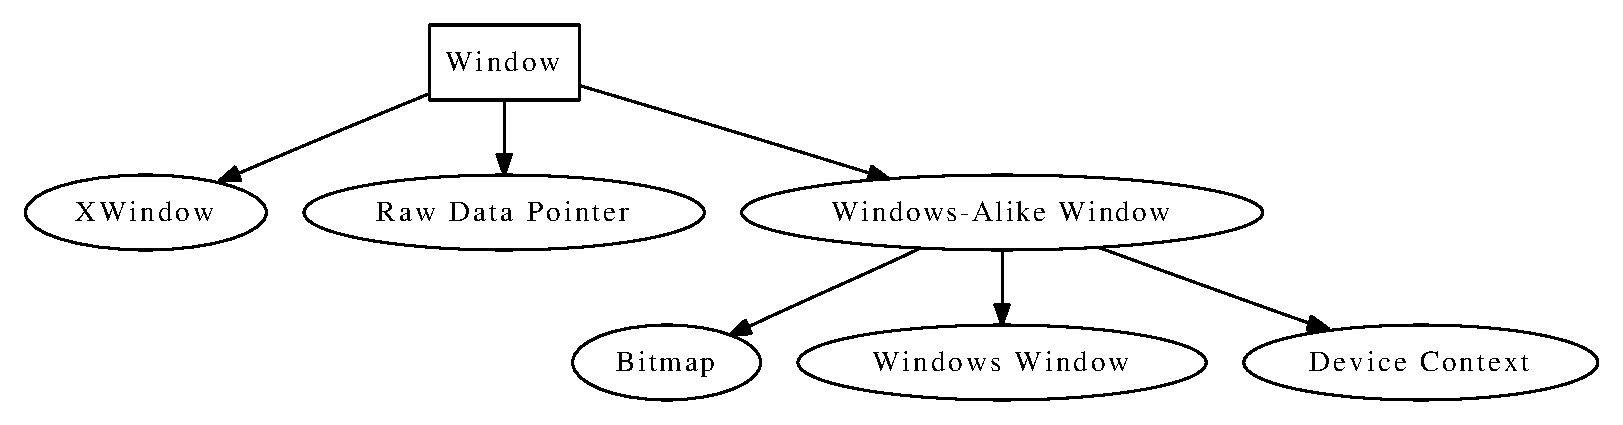
\includegraphics[scale=0.4]{Pics/Window_Types}
	\caption{Different types of Windows. Note that XWindow is only for non-Windows systems.}
\end{figure}

Figure 3 shows the three different Window Types supported by Mufasa.

Quick overview of functions:

\begin{itemize}
	\item ReturnData
	\item FreeReturnedData
	\item GetDimensions
	\item SetTargetWindow
	\item SetTargetIntArray
	\item SetTargetXWindow
	\item GetPixel
\end{itemize}

Together, these functions form the core of the window management, except for input.

\subsection{The Input Class}

The Input Class is the class that takes care of all the input.

\begin{figure}[h]
	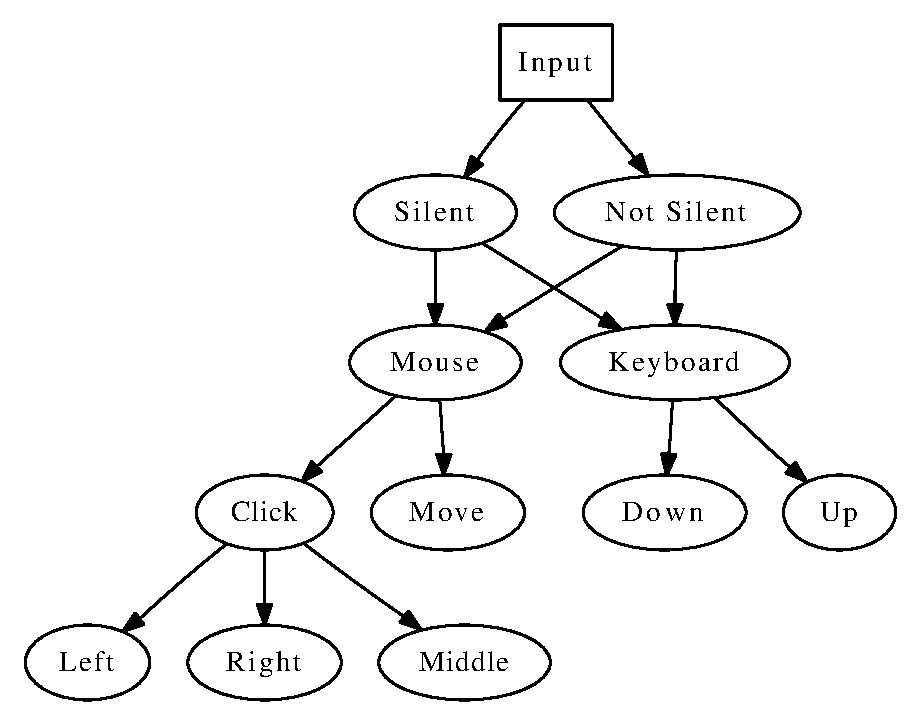
\includegraphics[scale=0.4]{Pics/Input_Diag}
	\caption{Input Functionality.}
\end{figure}

As one can see in Figure 4, MML aims to support both Silent and non Silent Input.
Since the Input heavily differs per operating system, the Input class should have a general way of sending keys, possibly at the expense of losing some functionality.

\subsection{The Color Convertions Include}

This .inc file contains pascal code to quickly convert one colour type to another.
It also adds support for comparing colours. The reason this is not a class, is because constantly dereferencing a class to call a single function doesn't do the speed of a program any good. There also wasn't really a need for a class, since none of these functions need to be initialized in any way.

\subsection{The Colour Class}

The colour class is a Class that does all the colour identfying and locating work. (FindColor, for example)
The colour class uses the Convertions include for several of it's functions.

A FindColor-derivative function in Mufasa exists generally out of the following steps:
\begin{itemize}
	\item Retrieve Client Data.
	\item Loop over the data, possibly with a special algorithm.
	\item Check the current pixel data against another colour, possibly with tolerance.
	\item Free the Client Data.
	\item Return found point(s).
\end{itemize}

\begin{figure}[h]
    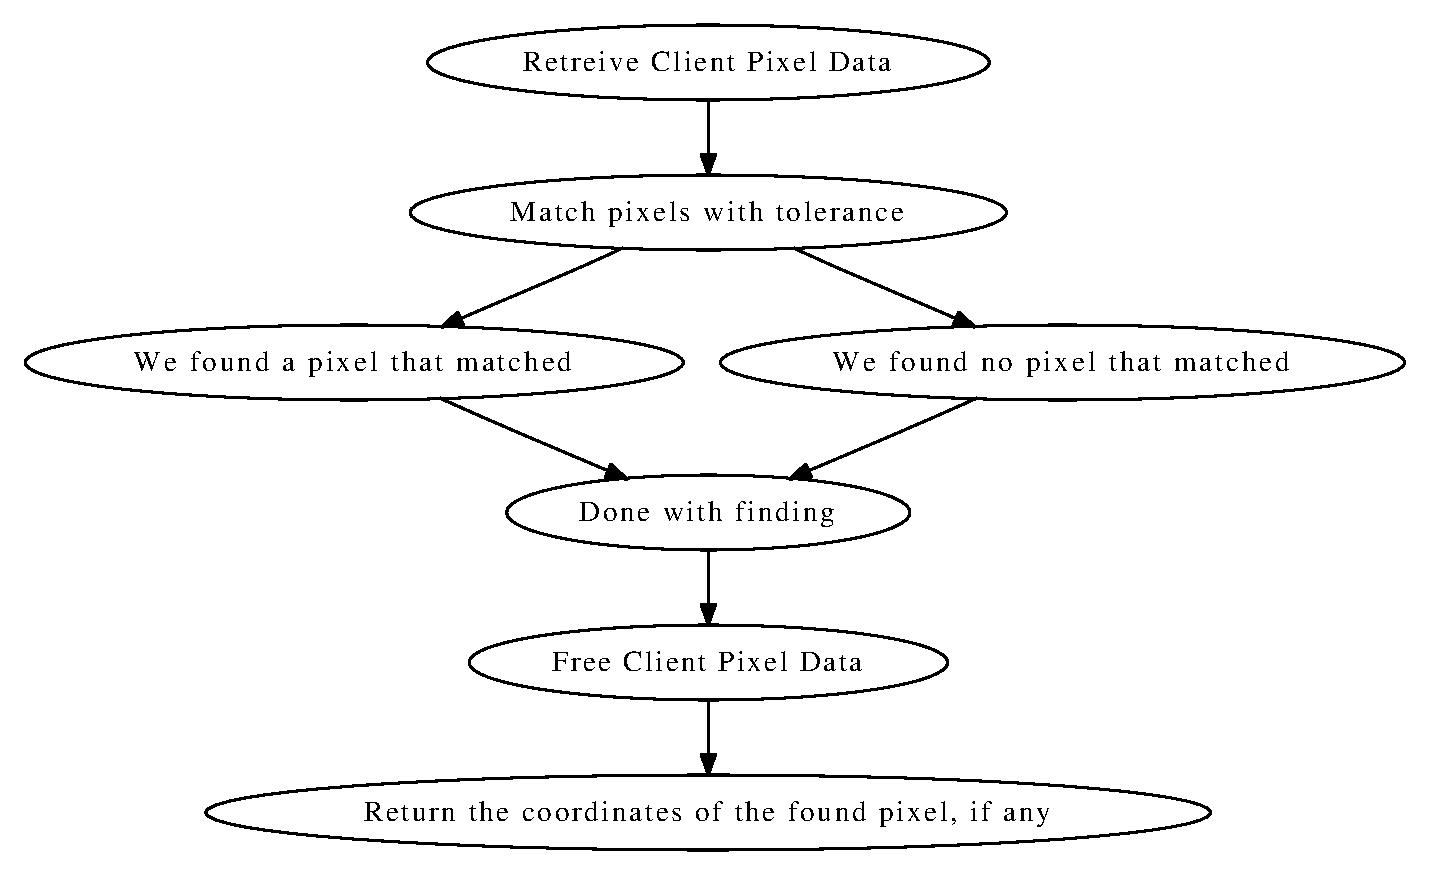
\includegraphics[scale=0.4]{Pics/FindColor}
    \caption{A basic find colour.}
\end{figure}

\subsection{Notes on the previously mentioned classes}

At this point it is unsure if the Input class will also take care of Sockets and Files. Most likely these will get their own class.

\section{More On The Core Classes}

The previously mentioned MML classes are considered to be the absolute core of the library. (Although one could argue that even the Colour class isn't part of the core classes.)
With these classes most functions that Mufasa will contain can be created. if you can make FindColor, you can make FindColorsSpiralTolerance, they don't really differ a lot. The same goes for DTM's, OCR and Bitmaps. Mouse and keyboard functions will be done with the Input class.

The MML contains more classes, and they will mainly utilize the previous mentioned classes.
It is essential to understand the Classes architecture to fully understand Mufasa.
Before work on other classes will be done, the core classes must be finished and stable.

\end{document}
